% (3 Seiten)
\section{Evaluation of the Classification Models}
\label{sec:ModelEval}
This section evaluates different classification models with three quality measures. These are the Precision $P$, the Recall $R$ and the $F_{\beta}$-Score, which are defined in Definition \ref{def_prf}. These quality measures are somewhat unrealistic for this use case since they do not take into account the collisions described in Section \ref{sec:NEL}. Therefore they will be compared with quality measures taking the collisions into account in Section \ref{sec:NELEval}.\par
Let $T$ be the set containing the feature entries to be classified. Each feature entry also has a label containing the result (positive or negative) the classifier should predict. The subsets $T_{TP}$, $T_{FP}$ and $T_{FN}$, which are used to calculate the quality measures, are defined as follows.\\
\begin{nscenter}
	$T_{TP} \subset T$, where $\forall f_e \in T_{TP}: f_e$ is labeled positive $\land$ $f_e$ is classified positive\\
	$T_{FP} \subset T$, where $\forall f_e \in T_{FP}: f_e$ is labeled negative $\land$ $f_e$ is classified positive\\
	$T_{FN} \subset T$, where $\forall f_e \in T_{FN}: f_e$ is labeled positive $\land$ $f_e$ is classified negative\\
\end{nscenter}
\begin{definition}
$P = \frac{\abs{T_{TP}}}{\abs{T_{TP} \ \cup \ T_{FP}}}$
$R = \frac{\abs{T_{TP}}}{\abs{T_{TP} \ \cup \ T_{FN}}}$
$F_{\beta} = \frac{(1 \ + \ \beta^2) \ \cdot \ P \ \cdot \ R}{(\beta^2 \ \cdot \ P) \ + \ R}$
\label{def_prf}
\end{definition}
% Precision, Recall reference: Cleverdon, C.W., Mills, J., and Keen, E.M. (1966). An inquiry in testing of information retrieval systems. (2 vols.). Cranfileld, U.K.: Aslib Cranfield Research Project, College of Aeronautics.
The following classification models will be tested: Naive Bayes, Logistic Regression, Gradient Boosted Trees and Random Forest. The implementations of the Apache Spark MLlib \footnote{https://spark.apache.org/mllib/} will be used. Specifically, the Data Frame API of Spark 2.1.0, since it is the primary API. The data set used to train and test the models is extracted from the Wikipedia pages $W_{business}$ as described in section 3. 70\% of the generated feature entries are used to train the model and the remaining 30\% are used to test it. Since the data set contains many more negative entries than positive entries it is very likely for a model to classify every feature entry as false. That way the model would still be correct in over 99\% of the cases. To mitigate this the training set is filtered by removing each entry having a rank $\geq 10$. This rank is the higher order feature of either the link score or the context score.\par
Figure \ref{classifier_eval} shows Precision, Recall and $F_1$-Score of the four tested models. Both the Naive Bayes and the Logistic Regression classified every feature entry as false resulting in a Precision and $F_1$-Score of NaN (due to division by 0). This is caused by too many negative input feature entries with not enough positive ones resulting in the classification of every input feature entry as false. Contrary to them, both the Gradient Boosted Trees and the Random Forest classified the data successfully. Only these two models use Decision Trees, showing that such unequal distributions of negative and positive input data are handled better by Decision Tree based models. The results of both are very similar, with the Random Forest having 2\% more Precision and the Gradient Boosted Trees having 6\% more Recall. Since the focus lies on the Precision the Random Forest was chosen for the feature evaluation in Section \ref{sec:FeatureEval}.\par
The Naive Bayes and Logistic Regression were both tested with different thresholds for the classes. A higher threshold means that the classifier needs to be more certain about a specific feature entry to classify it as positive. They were especially tested with very low threshold to see whether or not they would classify anything as positive. Unfortunately, this did not result in a different classification result. The Logistic Regression has a few more parameters other than the threshold. For these, the default values of the Spark MLlib were used.\par
\begin{figure}[H]
	\centering
	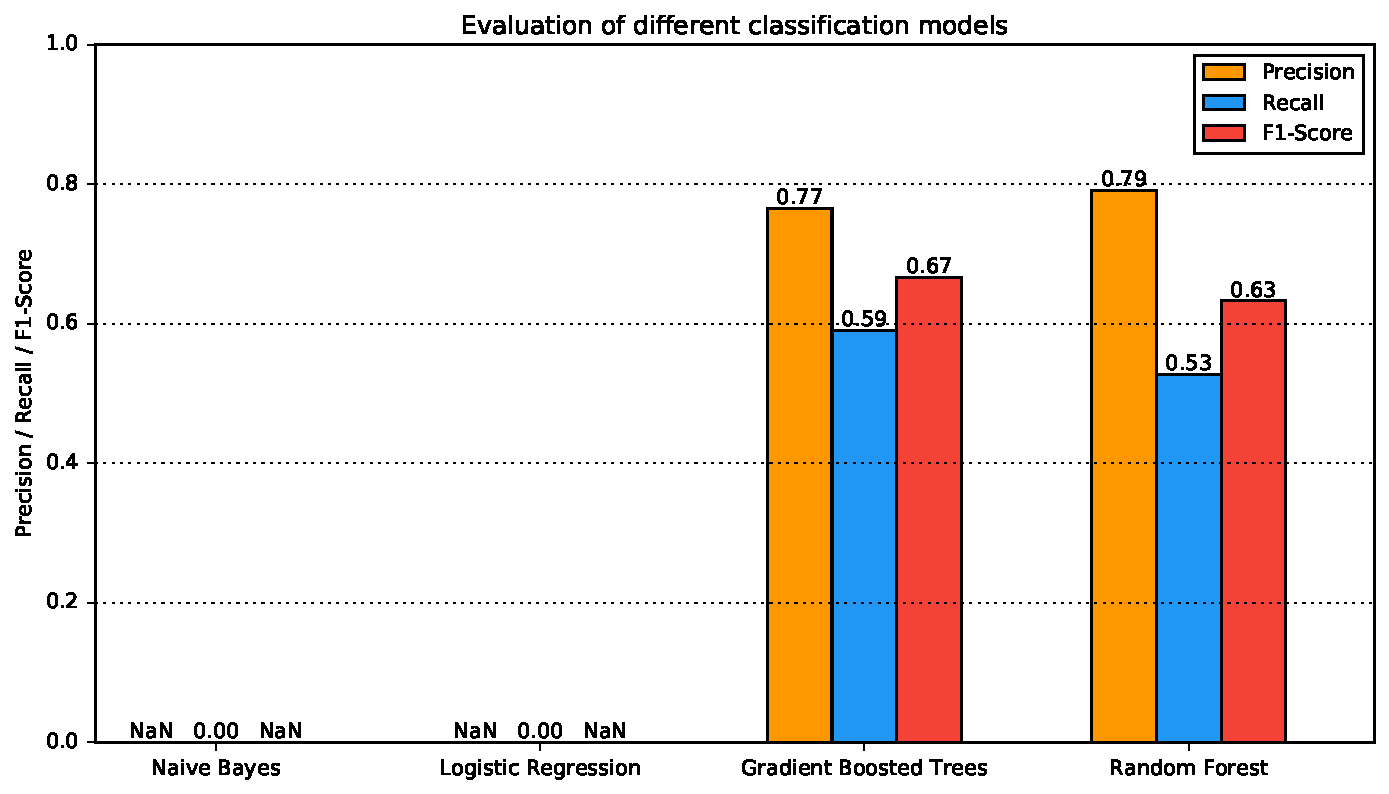
\includegraphics[width=\textwidth]{img/classifier_eval}
	\caption{Evaluation of different classification models.}
	\label{classifier_eval}
\end{figure}
The same parameters concerning the Decision Trees were used for the Gradient Boosted Trees and the Random Forest. These were 20 trees, a maximum depth of 6 and a maximum of 40 bins. The Gradient Boosted Trees were tested with a few different number of iterations. The values displayed in Figure \ref{classifier_eval} were the best for the tested number of iterations, which were 20. The other values resulted in a minimally worse Precision. The number of trees, the maximum depth and the maximum number of bins were tested using a Random Forest, but none of these parameters changed anything drastically.\par
Since the Spark MLlib does not provide a way to change the class thresholds, or rather the loss function, for Gradient Boosted Trees the evaluation of the class thresholds was done with a Random Forest. Figure \ref{rf_thresh_large} shows the behavior of the quality measures with a different threshold. The threshold of the model can be imagined as a threshold for the two classes, negative and positive. A higher threshold means that the classifier has to be more certain that a specific feature entry is positive and a lower threshold means that the classifier has to be less certain, which means that it is similar to a cost function. The threshold displayed in Figure \ref{rf_thresh_large} is a divisor of the just described threshold, meaning that e.g. the x value of $15.0$ results in the threshold being divided by $15.0$ and thus a very low threshold. In the following, a low threshold means a low threshold in Figure \ref{rf_thresh_large}, i.e. resulting in an actual higher threshold and vice versa.
\begin{figure}[H]
	\centering
	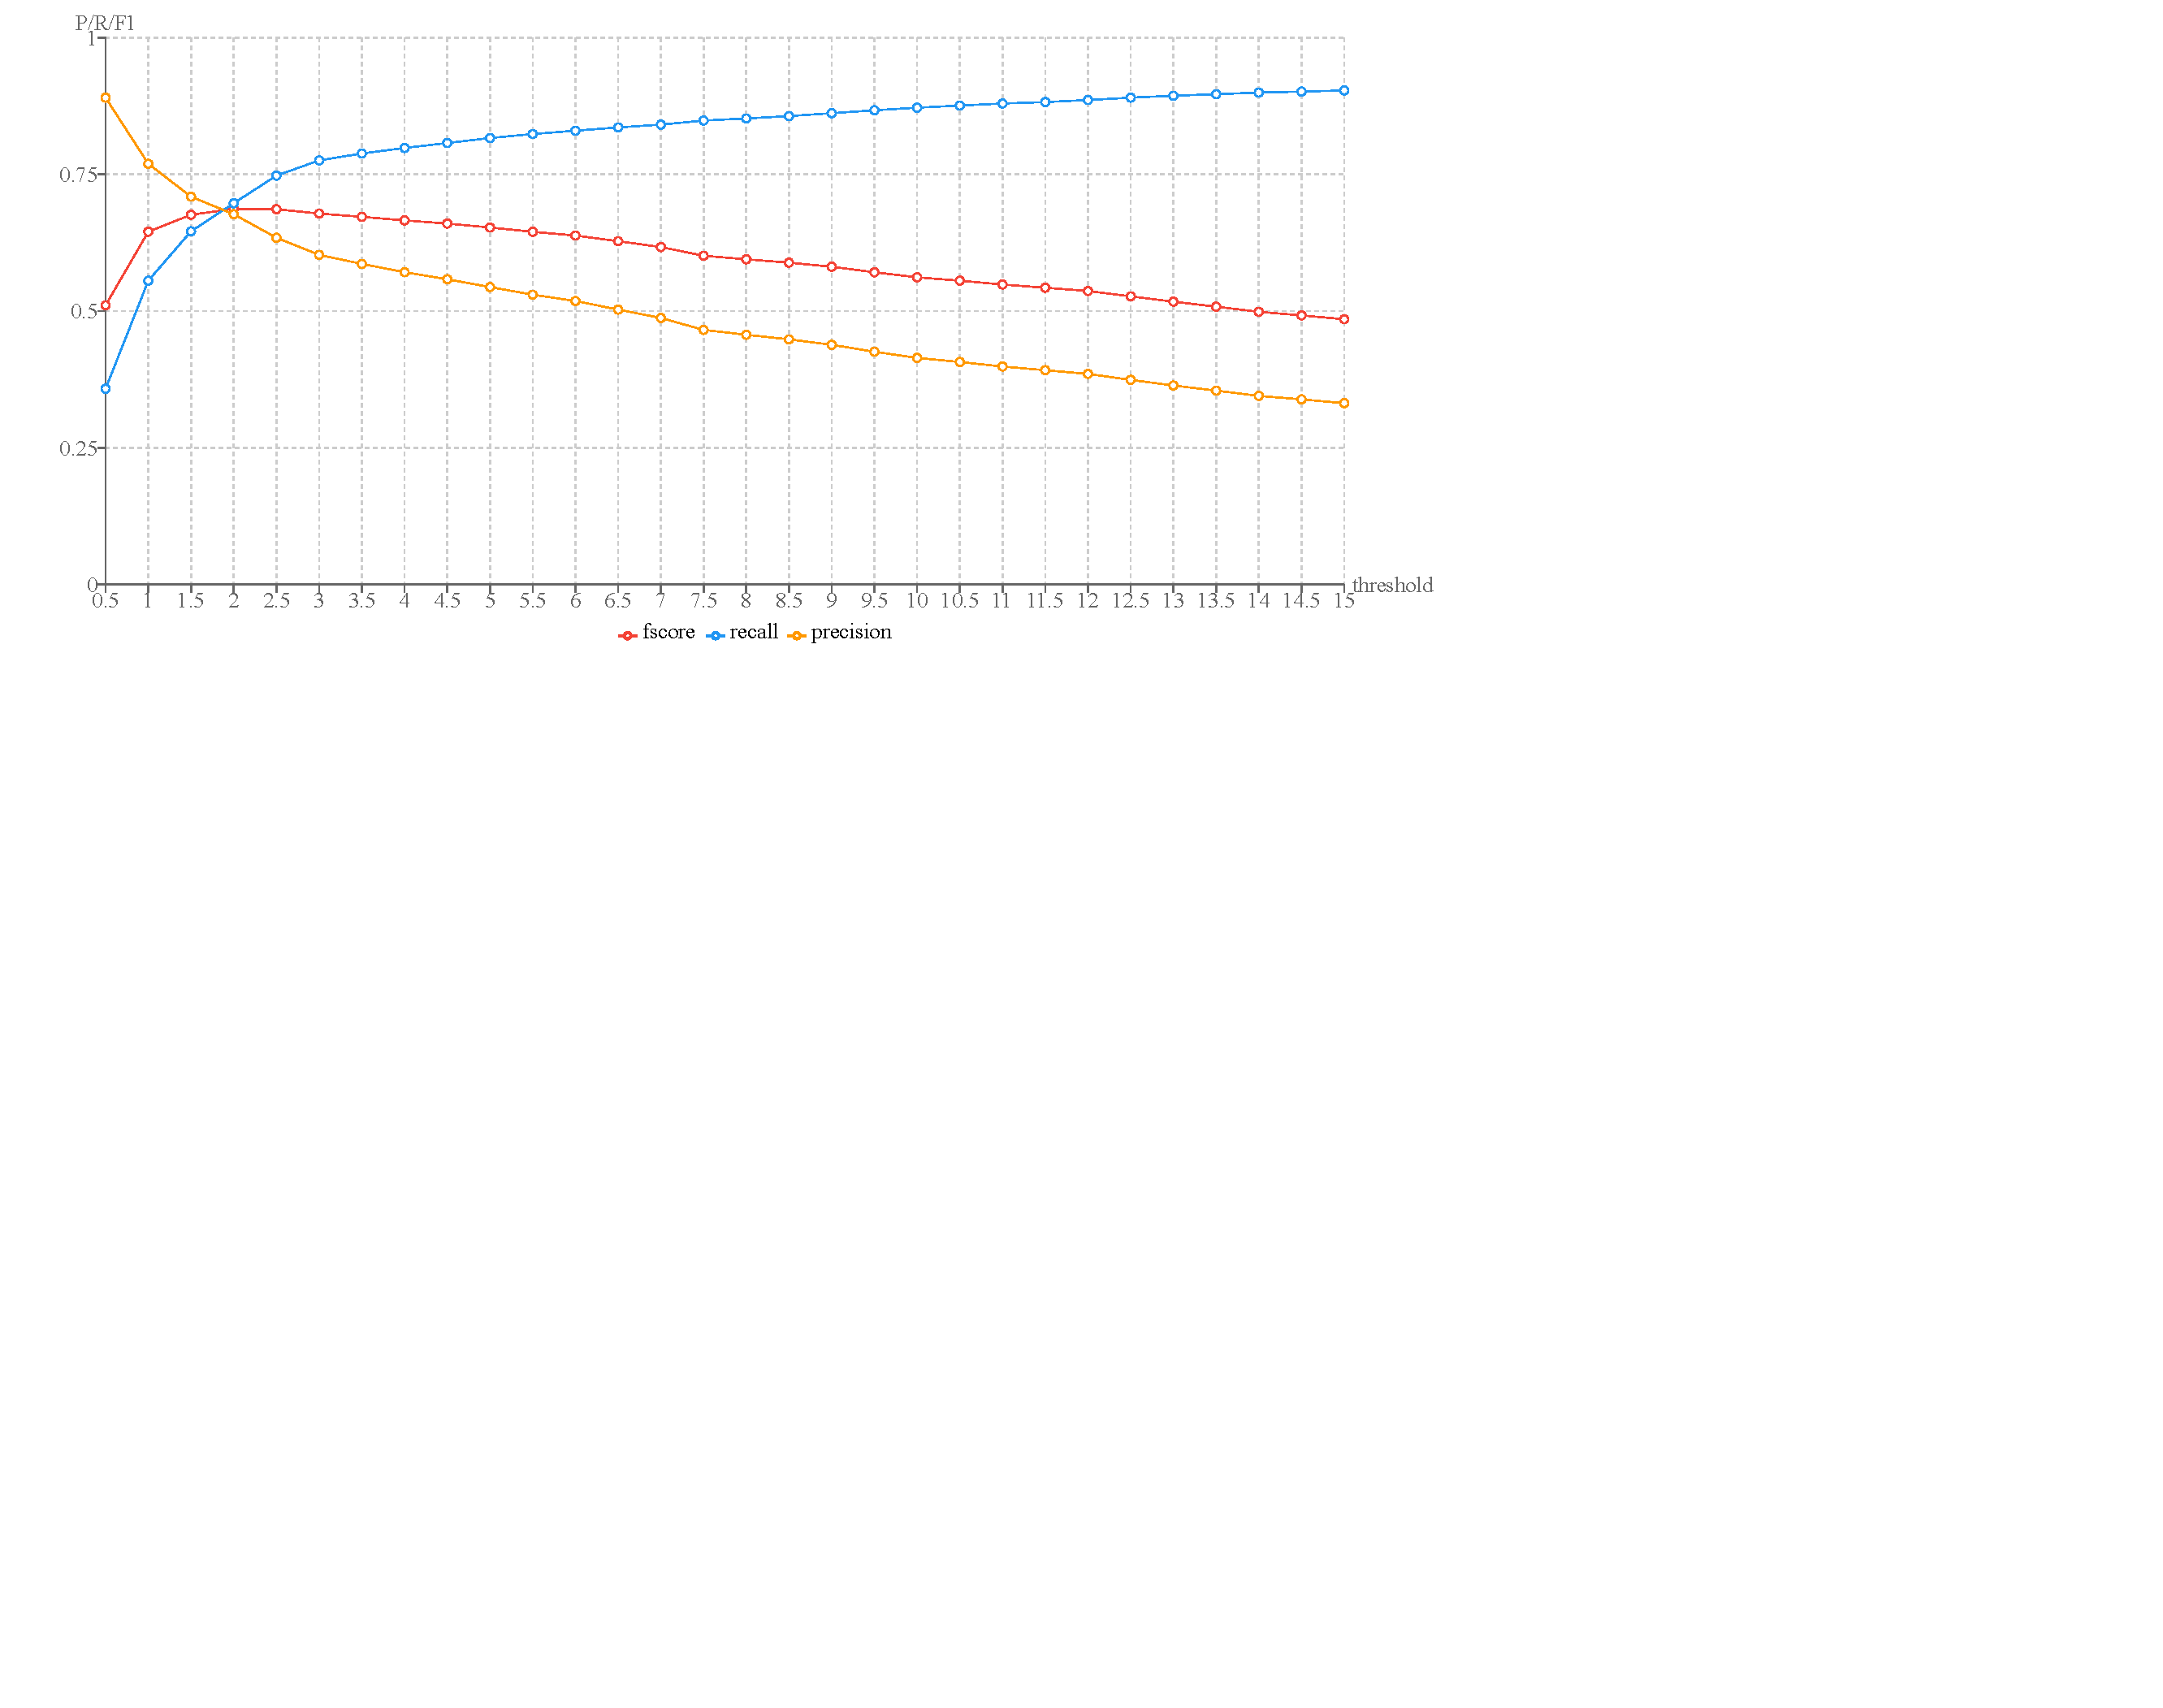
\includegraphics[width=\textwidth]{img/rf_thresh_large}
	\caption{Evaluation of different class thresholds of a random forest model.}
	\label{rf_thresh_large}
\end{figure}
It is visible that a low threshold results in a very high precision with a relatively low recall. The threshold of $0.5$ results in a Precision of $89\%$ and a Recall of $36\%$. A very high threshold leads to a higher Recall with a worse Precision. An $80\%$ Recall is achieved with a threshold of $4$, which has a Precision of $57\%$. A $90\%$ Recall is achieved with a threshold of $14.5$, which has a Precision of $34\%$. This shows that increasing the threshold has diminishing returns for the Recall while the drop of the Precision is relatively uniform. These thresholds can be used to create two classifiers, one with a high Precision but low Recall and one with a high Recall but a low Precision. As described by Grütze et al. \cite{coheel} these classifiers could be used in the future to create high-quality seed alignments with the high Precision classifier and high-coverage candidate alignments with the high Recall classifier. The candidate alignments could be used to increase the Recall of the seed alignments, e.g. by using Random Walks.


% Kurz erklären was man im Bild sieht\par
% Naive Bayes
% \begin{itemize}
% 	\item nimmt an die features seien unabhängig, was sie nicht sind
% 	\item sagt immer nein, da zu viele negative feature entries
% 	\item verschiedene Kostenmodelle/Gewichte getestet
% \end{itemize}
% Logistic Regression
% \begin{itemize}
% 	\item sagt immmer nein, da zu viele negative feature entries
% 	\item verschiedene Kostenmodelle getestet
% 	\item Standard Paramter der Spark ML lib (und des Beispiels) benutzt
% \end{itemize}
% Gradient Boosted Trees
% \begin{itemize}
% 	\item benutzte parameter
% 	\item Bei Iteration Parameter den minimal besten Wert bei 20 Iterationen (ein paar verschiedene Iterationen getestet)
% \end{itemize}
% Random Forest
% \begin{itemize}
	% \item vergleich DF und RDD API
% 	\item parameter getuned, haben aber nicht wirklich was geändert
% 	\item Kostenmodell kurve zeigen (für Seed und Candidate Alignments)
% \end{itemize}


% \begin{figure}[H]
% 	\centering
% 	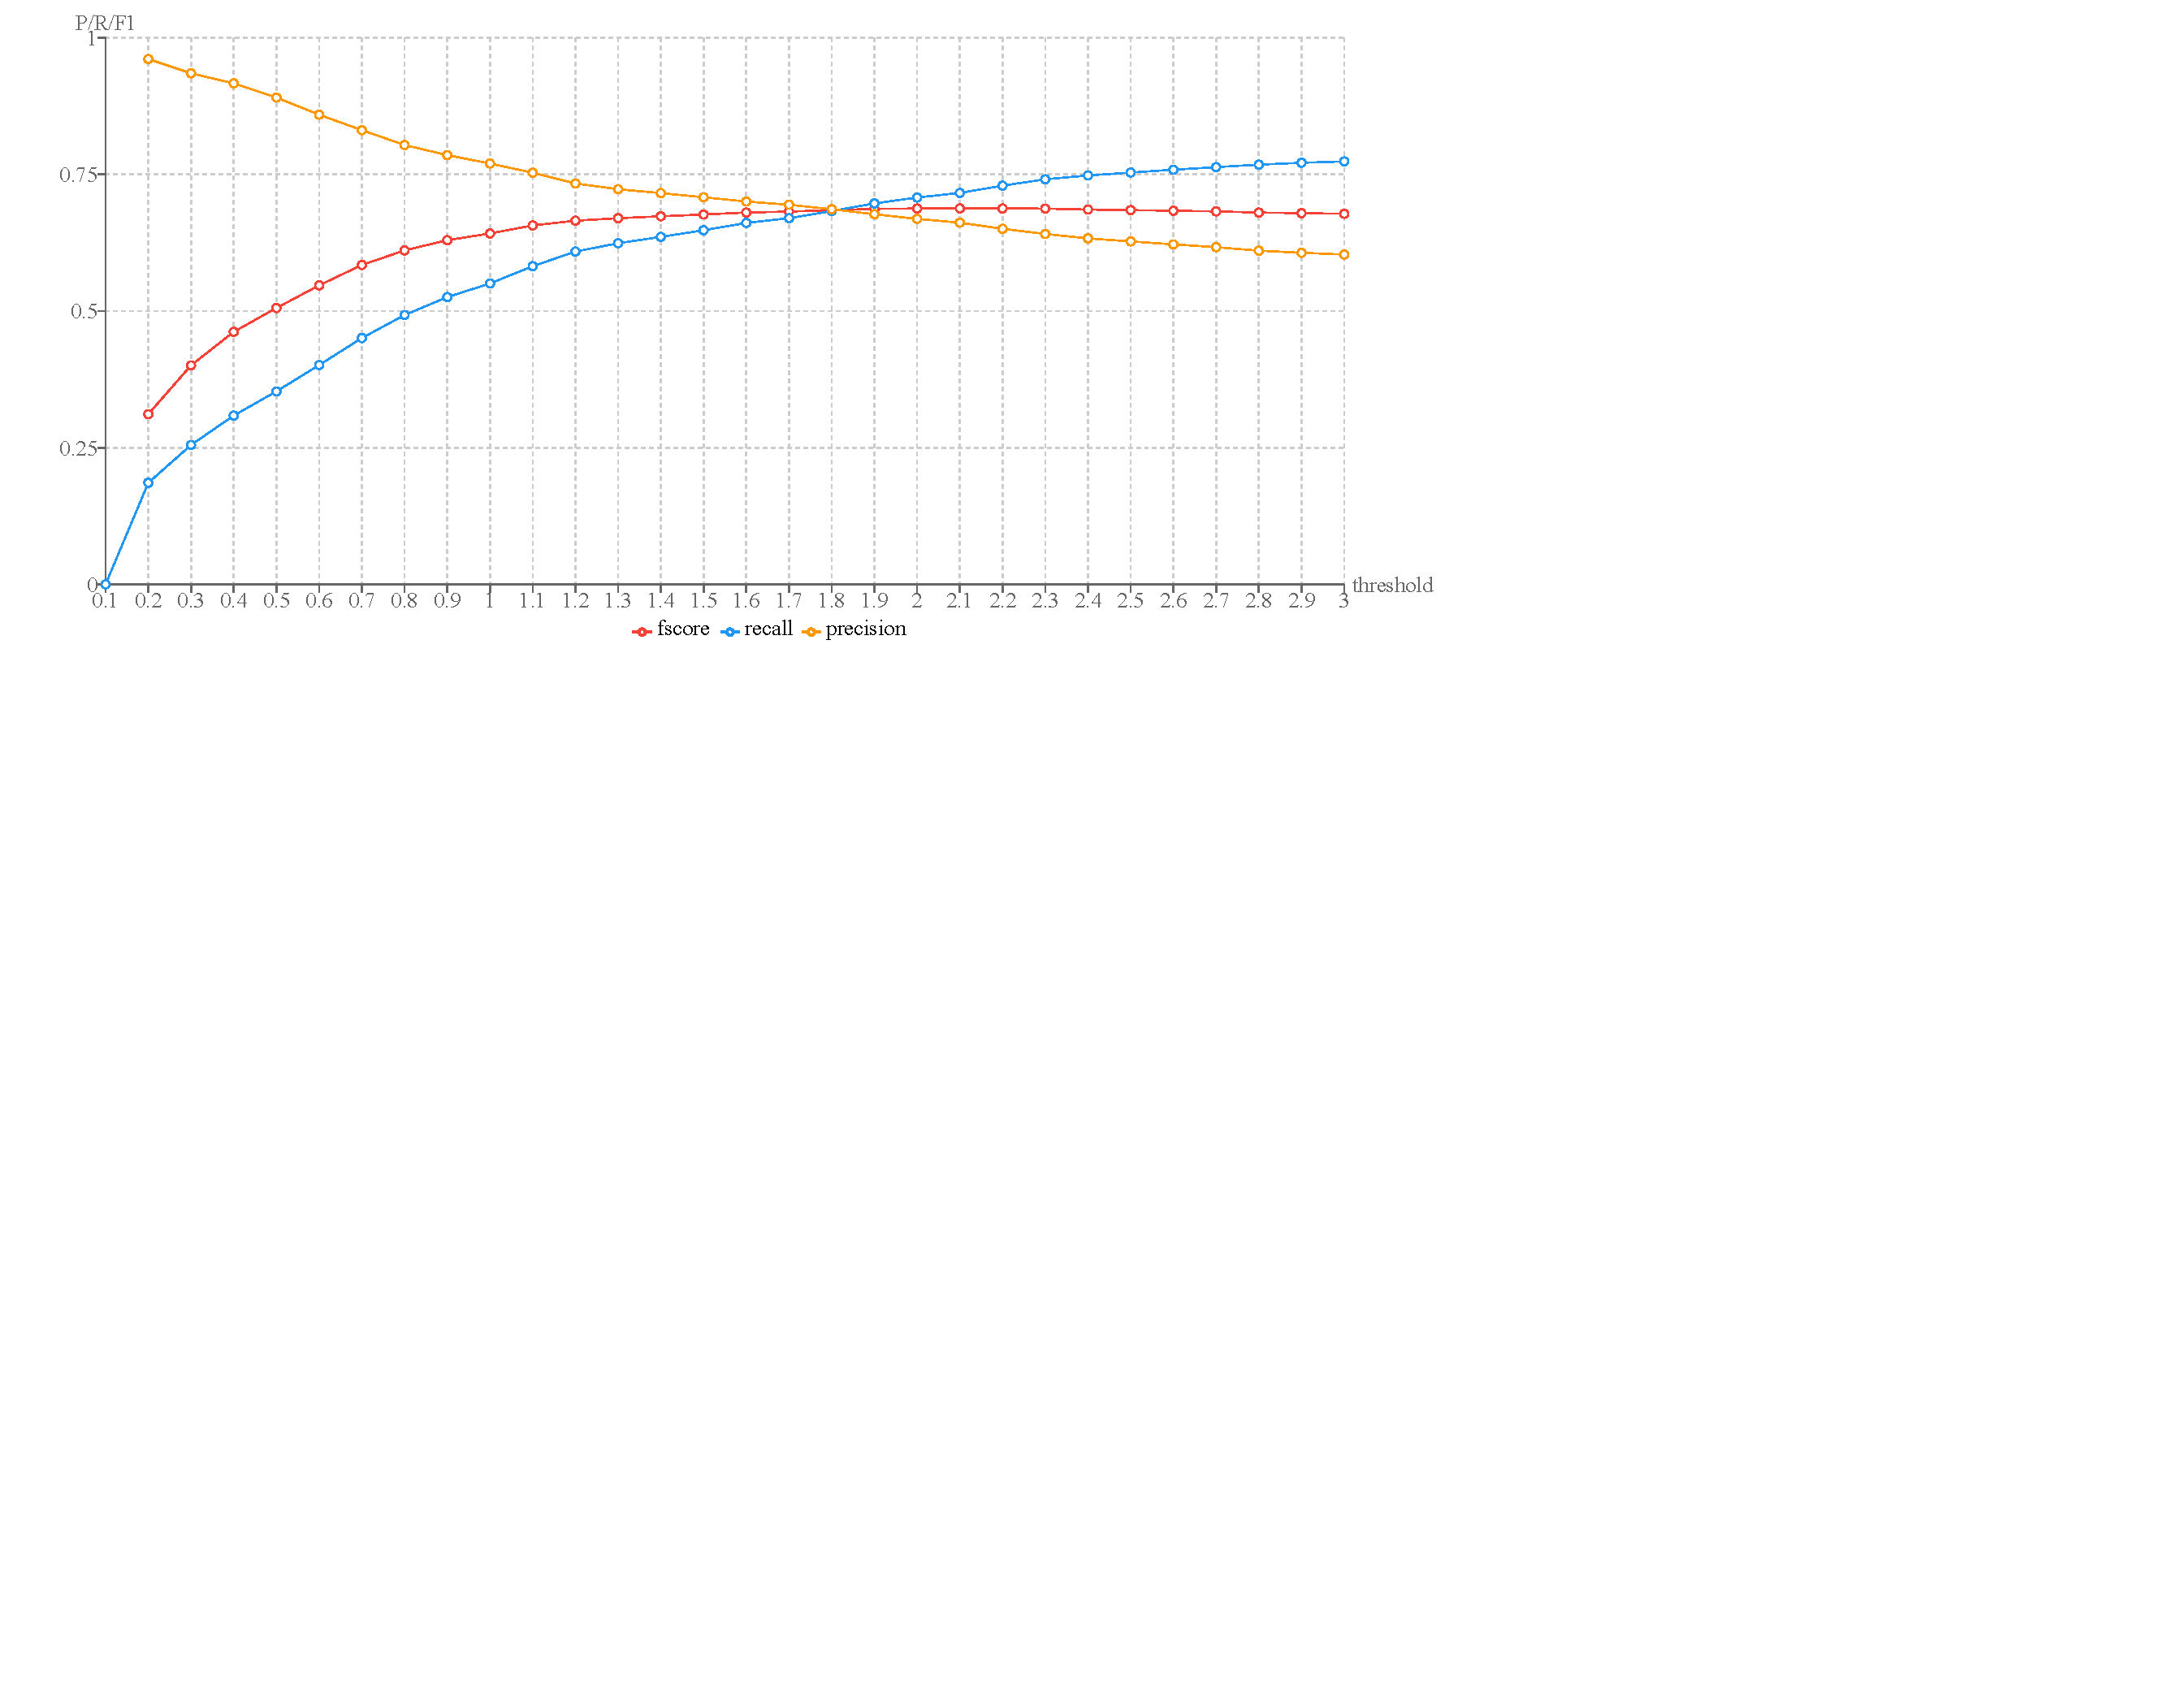
\includegraphics[width=\textwidth]{img/rf_thresh_small}
% 	\caption{Evaluation of different class weights of a random forest model.}
% 	\label{rf_thresh_small}
% \end{figure}

